\documentclass[]{book}
\usepackage{lmodern}
\usepackage{amssymb,amsmath}
\usepackage{ifxetex,ifluatex}
\usepackage{fixltx2e} % provides \textsubscript
\ifnum 0\ifxetex 1\fi\ifluatex 1\fi=0 % if pdftex
  \usepackage[T1]{fontenc}
  \usepackage[utf8]{inputenc}
\else % if luatex or xelatex
  \ifxetex
    \usepackage{mathspec}
  \else
    \usepackage{fontspec}
  \fi
  \defaultfontfeatures{Ligatures=TeX,Scale=MatchLowercase}
\fi
% use upquote if available, for straight quotes in verbatim environments
\IfFileExists{upquote.sty}{\usepackage{upquote}}{}
% use microtype if available
\IfFileExists{microtype.sty}{%
\usepackage{microtype}
\UseMicrotypeSet[protrusion]{basicmath} % disable protrusion for tt fonts
}{}
\usepackage[margin=1in]{geometry}
\usepackage{hyperref}
\hypersetup{unicode=true,
            pdftitle={EPIB 607: Inferential Statistics},
            pdfauthor={Sahir Bhatnagar and James Hanley},
            pdfborder={0 0 0},
            breaklinks=true}
\urlstyle{same}  % don't use monospace font for urls
\usepackage{natbib}
\bibliographystyle{apalike}
\usepackage{color}
\usepackage{fancyvrb}
\newcommand{\VerbBar}{|}
\newcommand{\VERB}{\Verb[commandchars=\\\{\}]}
\DefineVerbatimEnvironment{Highlighting}{Verbatim}{commandchars=\\\{\}}
% Add ',fontsize=\small' for more characters per line
\usepackage{framed}
\definecolor{shadecolor}{RGB}{248,248,248}
\newenvironment{Shaded}{\begin{snugshade}}{\end{snugshade}}
\newcommand{\KeywordTok}[1]{\textcolor[rgb]{0.13,0.29,0.53}{\textbf{#1}}}
\newcommand{\DataTypeTok}[1]{\textcolor[rgb]{0.13,0.29,0.53}{#1}}
\newcommand{\DecValTok}[1]{\textcolor[rgb]{0.00,0.00,0.81}{#1}}
\newcommand{\BaseNTok}[1]{\textcolor[rgb]{0.00,0.00,0.81}{#1}}
\newcommand{\FloatTok}[1]{\textcolor[rgb]{0.00,0.00,0.81}{#1}}
\newcommand{\ConstantTok}[1]{\textcolor[rgb]{0.00,0.00,0.00}{#1}}
\newcommand{\CharTok}[1]{\textcolor[rgb]{0.31,0.60,0.02}{#1}}
\newcommand{\SpecialCharTok}[1]{\textcolor[rgb]{0.00,0.00,0.00}{#1}}
\newcommand{\StringTok}[1]{\textcolor[rgb]{0.31,0.60,0.02}{#1}}
\newcommand{\VerbatimStringTok}[1]{\textcolor[rgb]{0.31,0.60,0.02}{#1}}
\newcommand{\SpecialStringTok}[1]{\textcolor[rgb]{0.31,0.60,0.02}{#1}}
\newcommand{\ImportTok}[1]{#1}
\newcommand{\CommentTok}[1]{\textcolor[rgb]{0.56,0.35,0.01}{\textit{#1}}}
\newcommand{\DocumentationTok}[1]{\textcolor[rgb]{0.56,0.35,0.01}{\textbf{\textit{#1}}}}
\newcommand{\AnnotationTok}[1]{\textcolor[rgb]{0.56,0.35,0.01}{\textbf{\textit{#1}}}}
\newcommand{\CommentVarTok}[1]{\textcolor[rgb]{0.56,0.35,0.01}{\textbf{\textit{#1}}}}
\newcommand{\OtherTok}[1]{\textcolor[rgb]{0.56,0.35,0.01}{#1}}
\newcommand{\FunctionTok}[1]{\textcolor[rgb]{0.00,0.00,0.00}{#1}}
\newcommand{\VariableTok}[1]{\textcolor[rgb]{0.00,0.00,0.00}{#1}}
\newcommand{\ControlFlowTok}[1]{\textcolor[rgb]{0.13,0.29,0.53}{\textbf{#1}}}
\newcommand{\OperatorTok}[1]{\textcolor[rgb]{0.81,0.36,0.00}{\textbf{#1}}}
\newcommand{\BuiltInTok}[1]{#1}
\newcommand{\ExtensionTok}[1]{#1}
\newcommand{\PreprocessorTok}[1]{\textcolor[rgb]{0.56,0.35,0.01}{\textit{#1}}}
\newcommand{\AttributeTok}[1]{\textcolor[rgb]{0.77,0.63,0.00}{#1}}
\newcommand{\RegionMarkerTok}[1]{#1}
\newcommand{\InformationTok}[1]{\textcolor[rgb]{0.56,0.35,0.01}{\textbf{\textit{#1}}}}
\newcommand{\WarningTok}[1]{\textcolor[rgb]{0.56,0.35,0.01}{\textbf{\textit{#1}}}}
\newcommand{\AlertTok}[1]{\textcolor[rgb]{0.94,0.16,0.16}{#1}}
\newcommand{\ErrorTok}[1]{\textcolor[rgb]{0.64,0.00,0.00}{\textbf{#1}}}
\newcommand{\NormalTok}[1]{#1}
\usepackage{longtable,booktabs}
\usepackage{graphicx,grffile}
\makeatletter
\def\maxwidth{\ifdim\Gin@nat@width>\linewidth\linewidth\else\Gin@nat@width\fi}
\def\maxheight{\ifdim\Gin@nat@height>\textheight\textheight\else\Gin@nat@height\fi}
\makeatother
% Scale images if necessary, so that they will not overflow the page
% margins by default, and it is still possible to overwrite the defaults
% using explicit options in \includegraphics[width, height, ...]{}
\setkeys{Gin}{width=\maxwidth,height=\maxheight,keepaspectratio}
\IfFileExists{parskip.sty}{%
\usepackage{parskip}
}{% else
\setlength{\parindent}{0pt}
\setlength{\parskip}{6pt plus 2pt minus 1pt}
}
\setlength{\emergencystretch}{3em}  % prevent overfull lines
\providecommand{\tightlist}{%
  \setlength{\itemsep}{0pt}\setlength{\parskip}{0pt}}
\setcounter{secnumdepth}{5}
% Redefines (sub)paragraphs to behave more like sections
\ifx\paragraph\undefined\else
\let\oldparagraph\paragraph
\renewcommand{\paragraph}[1]{\oldparagraph{#1}\mbox{}}
\fi
\ifx\subparagraph\undefined\else
\let\oldsubparagraph\subparagraph
\renewcommand{\subparagraph}[1]{\oldsubparagraph{#1}\mbox{}}
\fi

%%% Use protect on footnotes to avoid problems with footnotes in titles
\let\rmarkdownfootnote\footnote%
\def\footnote{\protect\rmarkdownfootnote}

%%% Change title format to be more compact
\usepackage{titling}

% Create subtitle command for use in maketitle
\newcommand{\subtitle}[1]{
  \posttitle{
    \begin{center}\large#1\end{center}
    }
}

\setlength{\droptitle}{-2em}

  \title{EPIB 607: Inferential Statistics}
    \pretitle{\vspace{\droptitle}\centering\huge}
  \posttitle{\par}
    \author{Sahir Bhatnagar and James Hanley}
    \preauthor{\centering\large\emph}
  \postauthor{\par}
      \predate{\centering\large\emph}
  \postdate{\par}
    \date{2018-09-05}

\usepackage{booktabs}
\usepackage{longtable}
\usepackage[bf,singlelinecheck=off]{caption}

\let\originaltabular\tabular
\let\endoriginaltabular\endtabular
\renewenvironment{tabular}[1]{%
  \begingroup%
  \centering%
  \originaltabular{#1}}%
  {\endoriginaltabular\endgroup}

\usepackage{ifxetex,ifluatex}
\usepackage{fixltx2e} % provides \textsubscript
\ifnum 0\ifxetex 1\fi\ifluatex 1\fi=0 % if pdftex
  \usepackage[$if(fontenc)$$fontenc$$else$T1$endif$]{fontenc}
  \usepackage[utf8]{inputenc}
\else % if luatex or xelatex
  \makeatletter
  \@ifpackageloaded{fontspec}{}{\usepackage{fontspec}}
  \makeatother
  \defaultfontfeatures{Ligatures=TeX,Scale=MatchLowercase}
  \makeatletter
  \@ifpackageloaded{soul}{
     \renewcommand\allcapsspacing[1]{{\addfontfeature{LetterSpace=15}#1}}
     \renewcommand\smallcapsspacing[1]{{\addfontfeature{LetterSpace=10}#1}}
   }{}
  \makeatother
\fi

\usepackage{graphicx}
\setkeys{Gin}{width=\linewidth,totalheight=\textheight,keepaspectratio}

\usepackage{units}

% multiplecol
\usepackage{multicol}

% strikeout
\usepackage[normalem]{ulem}

% morefloats
\usepackage{morefloats}

% tightlist macro required by pandoc >= 1.14
\providecommand{\tightlist}{%
  \setlength{\itemsep}{0pt}\setlength{\parskip}{0pt}}



%% -- tint overrides
%% fonts, using roboto (condensed) as default
\usepackage[sfdefault,condensed]{roboto}
%% also nice: \usepackage[default]{lato}

%% colored links, setting 'borrowed' from RJournal.sty with 'Thanks, Achim!'
\RequirePackage{color}
\definecolor{link}{rgb}{0.1,0.1,0.8} %% blue with some grey
\hypersetup{
  colorlinks,%
  citecolor=link,%
  filecolor=link,%
  linkcolor=link,%
  urlcolor=link
}


%\usepackage{fontspec}
%\setmainfont[UprightFeatures={SmallCapsFont=AlegreyaSC-Regular}]{Alegreya}

\usepackage{framed,color}
\definecolor{shadecolor}{RGB}{248,248,248}

\renewcommand{\textfraction}{0.05}
\renewcommand{\topfraction}{0.8}
\renewcommand{\bottomfraction}{0.8}
\renewcommand{\floatpagefraction}{0.75}

%\renewenvironment{quote}{\begin{VF}}{\end{VF}}
%\let\oldhref\href
%\renewcommand{\href}[2]{#2\footnote{\url{#1}}}

\ifxetex
  \usepackage{letltxmacro}
  \setlength{\XeTeXLinkMargin}{1pt}
  \LetLtxMacro\SavedIncludeGraphics\includegraphics
  \def\includegraphics#1#{% #1 catches optional stuff (star/opt. arg.)
    \IncludeGraphicsAux{#1}%
  }%
  \newcommand*{\IncludeGraphicsAux}[2]{%
    \XeTeXLinkBox{%
      \SavedIncludeGraphics#1{#2}%
    }%
  }%
\fi

\makeatletter
\newenvironment{kframe}{%
\medskip{}
\setlength{\fboxsep}{.8em}
 \def\at@end@of@kframe{}%
 \ifinner\ifhmode%
  \def\at@end@of@kframe{\end{minipage}}%
  \begin{minipage}{\columnwidth}%
 \fi\fi%
 \def\FrameCommand##1{\hskip\@totalleftmargin \hskip-\fboxsep
 \colorbox{shadecolor}{##1}\hskip-\fboxsep
     % There is no \\@totalrightmargin, so:
     \hskip-\linewidth \hskip-\@totalleftmargin \hskip\columnwidth}%
 \MakeFramed {\advance\hsize-\width
   \@totalleftmargin\z@ \linewidth\hsize
   \@setminipage}}%
 {\par\unskip\endMakeFramed%
 \at@end@of@kframe}
\makeatother

\renewenvironment{Shaded}{\begin{kframe}}{\end{kframe}}

\newenvironment{rmdblock}[1]
  {
  \begin{itemize}
  \renewcommand{\labelitemi}{
    \raisebox{-.7\height}[0pt][0pt]{
      {\setkeys{Gin}{width=3em,keepaspectratio}\includegraphics{images/#1}}
    }
  }
  \setlength{\fboxsep}{1em}
  \begin{kframe}
  \item
  }
  {
  \end{kframe}
  \end{itemize}
  }
\newenvironment{rmdnote}
  {\begin{rmdblock}{note}}
  {\end{rmdblock}}
\newenvironment{rmdcaution}
  {\begin{rmdblock}{caution}}
  {\end{rmdblock}}
\newenvironment{rmdimportant}
  {\begin{rmdblock}{important}}
  {\end{rmdblock}}
\newenvironment{rmdtip}
  {\begin{rmdblock}{tip}}
  {\end{rmdblock}}
\newenvironment{rmdwarning}
  {\begin{rmdblock}{warning}}
  {\end{rmdblock}}

\usepackage{makeidx}
\makeindex

\urlstyle{tt}

\usepackage{amsthm}
\makeatletter
\def\thm@space@setup{%
  \thm@preskip=8pt plus 2pt minus 4pt
  \thm@postskip=\thm@preskip
}
\makeatother




%\usepackage[pagebackref=false,bookmarks]{hyperref}
\hypersetup{
	unicode=false,          
	pdftoolbar=true,        
	pdfmenubar=true,        
	pdffitwindow=false,     % window fit to page when opened
	pdfstartview={FitH},    % fits the width of the page to the window
	pdftitle={EPIB 607 Notes},    % title
	pdfauthor={Sahir Rai Bhatnagar},     % author
	pdfsubject={Subject},   % subject of the document
	pdfcreator={Sahir Rai Bhatnagar},   % creator of the document
	pdfproducer={Sahir Rai Bhatnagar}, % producer of the document
	pdfkeywords={}, % list of keywords
	pdfnewwindow=true,      % links in new window
	colorlinks=true,       % false: boxed links; true: colored links
	linkcolor=red,          % color of internal links (change box color with linkbordercolor)
	citecolor=blue,        % color of links to bibliography
	filecolor=black,      % color of file links
	urlcolor=blue         % color of external links
}


%\frontmatter % turns off chapter numbering and uses roman numerals for page numbers;
% https://tex.stackexchange.com/questions/20538/what-is-the-right-order-when-using-frontmatter-tableofcontents-mainmatter

\usepackage{amsthm}
\newtheorem{theorem}{Theorem}[chapter]
\newtheorem{lemma}{Lemma}[chapter]
\theoremstyle{definition}
\newtheorem{definition}{Definition}[chapter]
\newtheorem{corollary}{Corollary}[chapter]
\newtheorem{proposition}{Proposition}[chapter]
\theoremstyle{definition}
\newtheorem{example}{Example}[chapter]
\theoremstyle{definition}
\newtheorem{exercise}{Exercise}[chapter]
\theoremstyle{remark}
\newtheorem*{remark}{Remark}
\newtheorem*{solution}{Solution}
\begin{document}
\maketitle

{
\setcounter{tocdepth}{1}
\tableofcontents
}
\part{Preface}\label{part-preface}

\chapter{Welcome}\label{welcome}

Welcome to the course notes for
\href{https://www.mcgill.ca/study/2018-2019/courses/epib-607}{EPIB 607:
Inferential Statistics} at McGill University.

\section{Objectives}\label{objectives}

The aim of this course is to provide students with basic principles of
statistical inference so that they can:

\begin{enumerate}
\def\labelenumi{\arabic{enumi}.}
\tightlist
\item
  Understand the statistical methods section in a scientific paper.\\
\item
  Apply statistical methods in their own research.\\
\item
  Use the methods learned in this course as a foundation for more
  advanced biostatistics courses.
\end{enumerate}

\section{Audience}\label{audience}

The principle audience is researchers in the natural and social sciences
who have a basic understanding of differentiable and integral calculus,
but haven't had an introductory course in statistics. This audience
accepts that statistics has penetrated the life sciences pervasively and
is required knowledge for both doing research and understanding
scientific papers.

\section{About these notes}\label{about-these-notes}

These notes are a collection of useful links, videos, online resources
and papers for an introductory course in statistics. The instructors
have found that no single book sufficiently teaches all the topics
covered in this course. Part of this is due to advancements in computing
which have far outpaced the publication of modern textbooks. Indeed, the
computer has replaced many of the calculations that were traditionally
taught to be done by hand. We direct the readers to what we think is a
good learning resource for a given topic (following the \textbf{Flipped
Classroom} strategy). We also provide our own commentary and notes when
we think its useful.

\section{R Code Conventions}\label{r-code-conventions}

We use \href{https://cran.r-project.org/}{\texttt{R}} code throughout
these notes. When \texttt{R} code is displayed\footnote{\url{https://raw.githubusercontent.com/coatless/spm/master/index.Rmd}}
it will be typeset using a \texttt{monospace} font with syntax
highlighting enabled to ensure the differentiation of functions,
variables, and so on. For example, the following adds 1 to 1

\begin{Shaded}
\begin{Highlighting}[]
\NormalTok{a =}\StringTok{ }\NormalTok{1L }\OperatorTok{+}\StringTok{ }\NormalTok{1L}
\NormalTok{a}
\end{Highlighting}
\end{Shaded}

Each code segment may contain actual output from \texttt{R}. Such output
will appear in grey font prefixed by \texttt{\#\textgreater{}}. For
example, the output of the above code segment would look like so:

\begin{verbatim}
[1] 2
\end{verbatim}

\section{Rendering Mathematical
Formulae}\label{rendering-mathematical-formulae}

Throughout these notes, there will be mathematical symbols used to
express the material. Depending on the version of the book, there are
two different rendering engines.

\begin{itemize}
\tightlist
\item
  For the online version, the text uses
  \href{https://www.mathjax.org/}{MathJax} to render mathematical
  notation for the web. In the event the formulae does not load for a
  specific chapter, first try to refresh the page. 9 times out of 10 the
  issue is related to the software library not loading quickly. You can
  also right-click to see the corresponding LaTeX code used to produce
  the equation.\\
\item
  For the pdf version, the text is built using the recommended AMS LaTeX
  symbolic packages. As a result, there should be no issue displaying
  equations. An example of a mathematical rendering capabilities would
  be given as:
\end{itemize}

\[ a^2 + b^2 = c^2 \]

\section{Development}\label{development}

This book is built with
\href{https://github.com/rstudio/bookdown}{\textbf{bookdown}} and is
open source and freely available. This approach encourages
contributions, ensures reproducibility and provides access to the
material worldwide. The online version of the book is hosted at
\href{https://sahirbhatnagar.com/EPIB607}{sahirbhatnagar.com/EPIB607}
and kept up-to-date thanks to
\href{https://travis-ci.org/sahirbhatnagar/EPIB607}{Travis}. The entire
source code is available at
\url{https://github.com/sahirbhatnagar/EPIB607}.

If you notice any errors, we would be grateful if you would let us know
by filing an issue
\href{https://github.com/sahirbhatnagar/EPIB607/issues}{here} or making
a pull request by clicking the edit button in the top-left corner of the
text:

\begin{figure}
\centering

\includegraphics{images/edit_button.png}
\caption{}
\end{figure}

The version of the book you are reading now was built on 2018-09-05 and
was built on
\href{https://travis-ci.org/sahirbhatnagar/MATH697}{Travis}.

\section{About the authors}\label{about-the-authors}

\begin{longtable}[]{@{}cc@{}}
\toprule
Sahir Bhatnagar & James Hanley\tabularnewline
\midrule
\endhead
&\tabularnewline
\bottomrule
\end{longtable}

\begin{itemize}
\tightlist
\item
  Sahir R. Bhatnagar: Assistant Professor of Biostatistics - McGill
  University, Montreal, Canada.

  \begin{itemize}
  \tightlist
  \item
    Website: \url{https://sahirbhatnagar.com/}\\
  \item
    Twitter: \href{https://twitter.com/syfi_24}{syfi\_24}\\
  \item
    GitHub: \url{https://github.com/sahirbhatnagar}\\
  \end{itemize}
\item
  James A. Hanley: Professor of Biostatistics - McGill University,
  Montreal, Canada.

  \begin{itemize}
  \tightlist
  \item
    Webpage: \url{http://www.medicine.mcgill.ca/epidemiology/hanley/}
  \end{itemize}
\end{itemize}

\section{License}\label{license}

This work is licensed under a Creative Commons Attribution 4.0
International License

\chapter{Course Information}\label{course-information}

\begin{itemize}
\tightlist
\item
  Instructor: \href{mailto:sahir.bhatnagar@mcgill.ca}{Sahir Bhatnagar}\\
\item
  Teaching Assistants: \href{mailto:kody.crowell1598@gmail.com}{Kody
  Crowell}, \href{mailto:guanbo.wang@mail.mcgill.ca}{Guanbo Wang},
  \href{mailto:dewdunee.marasinghe@mail.mcgill.ca}{Himasara
  Marasinghe}\\
\item
  Website: \url{http://sahirbhatnagar.com/EPIB607/}\\
\item
  Lectures: Monday 11:30am - 1:30pm, Thursday 8:30am - 10:30am\\
\item
  Location: McMed 1034\\
\item
  Office Hours: TBD\\
\item
  Prerequisite(s): Calculus and Algebra\\
\item
  Texts: \emph{The Practice of Statistics in the Life Sciences}, 3nd
  Edition by Baldi \& Moore.
\end{itemize}

\section{Teaching strategy}\label{teaching-strategy}

This course will follow the \textbf{Flipped Classroom} model. Here,
students are expected to have engaged with the material before coming to
class (based on very precise pre-class instructions). The students will
then be expected to answer a series of conceptual multiple choice
questions using the
\href{https://mydalite.org/en/live/signup/form/NTc4}{DALITE} online
platform \citep{bhatnagar2016dalite}.

This allows the instructor to delegate the delivery of basic content and
definitions to textbooks and videos, and enforces the idea that students
cannot be simply passive recipients of information. This approach then
allows the professor to focus valuable class time on nurturing efficient
discussions surrounding the ideas within the content, guiding
interactive exploration of typical misconceptions, and promoting
collaborative problem solving with peers.

\section{A focus on computation}\label{a-focus-on-computation}

Classic introductory statistics textbooks were written during a time
when computers were still in their infancy. As such, even the newer
editions heavily rely on \emph{by-hand} computations such as looking up
tables for tail probabilities. We take a modern approach and introduce
computational methods in statistics with the statistical software
program \texttt{R}.

\section{DataCamp}\label{datacamp}

This class is supported by \href{https://www.datacamp.com/}{DataCamp},
the most intuitive learning platform for data science. Learn R, Python
and SQL the way you learn best through a combination of short expert
videos and hands-on-the-keyboard exercises. Take over 100+ courses by
expert instructors on topics such as importing data, data visualization
or machine learning and learn faster through immediate and personalised
feedback on every exercise.

\begin{figure}
\centering

\includegraphics{images/datacamp.png}
\caption{}
\end{figure}

You will be asked to complete some of the courses in DataCamp for
background reading or for assignments. You can sign up for a free
account at
\href{https://www.datacamp.com/groups/shared_links/4c7d78a632b557dfdd6618b3e8fac09495571fec}{this
link}. Note: you are required to sign up with a \texttt{@mail.mcgill.ca}
or \texttt{@mcgill.ca} email address.

\section{Grade Distribution}\label{grade-distribution}

\begin{tabular}{ll}
\toprule
 & \\
\midrule
Assignments & 30\%\\
DALITE Quizzes & 10\%\\
Midterm & 20\%\\
Project & 10\%\\
Final Exam & 30\%\\
\bottomrule
\end{tabular}

\chapter{Target Syllabus}\label{target-syllabus}

\begin{tabular}{ll}
\toprule
Abbreviation & Description\\
\midrule
JH & James Hanley notes\\
EM & Erica Moodie notes\\
OS & Olli Saarela notes\\
AAO & Against all odds video series\\
B\&M & The practice of statistics in the life sciences by Baldi and Moore, 3rd edition\\
\addlinespace
Freedman & Statistics by Freedman, Pisani, Purves, Adhikari, 2nd edition\\
dataviz & Fundamentals of Data Visualization by Claus O. Wilke\\
\bottomrule
\end{tabular}

\section{Descriptive Statistics}\label{descriptive-statistics}

\begin{tabular}{lllll}
\toprule
Topic & Video & Readings & Exercise & DALITE\\
\midrule
Histograms & [AAO unit 3](https://www.learner.org/courses/againstallodds/unitpages/unit03.html) & [AAO unit 3, pages 1-6](https://www.learner.org/courses/againstallodds/pdfs/AgainstAllOdds\_StudentGuide\_Unit03.pdf\#page=1) & [AAO unit 3, Wafer Thickness pages 15-17](https://www.learner.org/courses/againstallodds/pdfs/AgainstAllOdds\_StudentGuide\_Unit03.pdf\#page=15) & --\\
Density Plots & -- & [dataviz chapter 7](https://serialmentor.com/dataviz/histograms-density-plots.html) & -- & --\\
Measures of Center & [AAO unit 4](https://www.learner.org/courses/againstallodds/unitpages/unit04.html) & [AAO unit 4, pages 1-6](https://www.learner.org/courses/againstallodds/pdfs/AgainstAllOdds\_StudentGuide\_Unit04.pdf\#page=1) & [AAO unit 4, Mean, Median and Distribution Shape pages 13-14](https://www.learner.org/courses/againstallodds/pdfs/AgainstAllOdds\_StudentGuide\_Unit04.pdf\#page=13) & --\\
Boxplots & [AAO unit 5](https://www.learner.org/courses/againstallodds/unitpages/unit05.html) & [AAO unit 5, pages 1-5](https://www.learner.org/courses/againstallodds/pdfs/AgainstAllOdds\_StudentGuide\_Unit05.pdf\#page=1) & -- & --\\
Standard Deviation & [AAO unit 6](https://www.learner.org/courses/againstallodds/unitpages/unit06.html) & [AAO unit 6, pages 1-3](https://www.learner.org/courses/againstallodds/pdfs/AgainstAllOdds\_StudentGuide\_Unit06.pdf\#page=1) & [AAO unit 4, Visualizing Standard Deviation pages 10-13](https://www.learner.org/courses/againstallodds/pdfs/AgainstAllOdds\_StudentGuide\_Unit06.pdf\#page=10) & --\\
Data Visualization & [Hans Rosling BBC](https://www.youtube.com/watch?v=jbkSRLYSojo) & -- & -- & --\\
\bottomrule
\end{tabular}

\section{Sampling Distributions}\label{sampling-distributions}

\begin{tabular}{lllll}
\toprule
Topic & Video & Readings & Exercise & DALITE\\
\midrule
Parameters and Statistics & -- & [[JH section 1]](https://www.dropbox.com/s/kr293cablb11nrm/Ch13SamplingDistributionsJH2018.pdf?dl=0) [[B\&M page 314]](https://www.dropbox.com/s/8u0j9lupv5pxqpm/Ch13SamplingDistributions.pdf?dl=0) & -- & --\\
Sampling Distributions & [AAO unit 22](https://www.learner.org/courses/againstallodds/unitpages/unit22.html) & [[AAO unit 22, pages 1-10]](https://www.learner.org/courses/againstallodds/pdfs/AgainstAllOdds\_StudentGuide\_Unit22.pdf) [[JH sections 2-6]](https://www.dropbox.com/s/kr293cablb11nrm/Ch13SamplingDistributionsJH2018.pdf?dl=0) [[B\&M pages 315-320]](https://www.dropbox.com/s/8u0j9lupv5pxqpm/Ch13SamplingDistributions.pdf?dl=0) & -- & --\\
Central Limit Theorem & [AAO unit 22](https://www.learner.org/courses/againstallodds/unitpages/unit22.html) & [B\&M pages 321-324](https://www.dropbox.com/s/8u0j9lupv5pxqpm/Ch13SamplingDistributions.pdf?dl=0) & -- & --\\
The Bootstrap & -- & [[Computer-Intensive Methods in Statistics]](http://folk.uio.no/deilerts/phd/docs/Efron-scientificamerican0583-116.pdf) [[Bootstrap confidence intervals ]](http://mosaic-web.org/go/SM2-technique/confidence-intervals.html) & -- & --\\
\bottomrule
\end{tabular}

\section{Introduction to Inference}\label{introduction-to-inference}

\begin{tabular}{lllll}
\toprule
Topic & Video & Readings & Exercise & DALITE\\
\midrule
Confidence Intervals & [AAO unit 24](https://www.learner.org/courses/againstallodds/unitpages/unit24.html) & [[AAO unit 24, pages 1-6]](https://www.learner.org/courses/againstallodds/pdfs/AgainstAllOdds\_StudentGuide\_Unit24.pdf) [[JH notes]](https://www.dropbox.com/s/epgqkz3g0qklcp9/Ch14ConfidenceIntervalsJH2018.pdf?dl=0) [[Standard deviation, standard error. Which 'standard' should we use?]](http://www.medicine.mcgill.ca/epidemiology/hanley/BionanoWorkshop/SD-SE.pdf) & -- & --\\
Tests of Significance and P-values & [AAO unit 25](https://www.learner.org/courses/againstallodds/unitpages/unit25.html) & [[AAO unit 25, pages 1-12]](https://www.learner.org/courses/againstallodds/pdfs/AgainstAllOdds\_StudentGuide\_Unit25.pdf) [[JH, What the p-value is not]](http://www.medicine.mcgill.ca/epidemiology/hanley/BionanoWorkshop/P-Values.pdf) & -- & --\\
\bottomrule
\end{tabular}

\section{One-sample Inference}\label{one-sample-inference}

\begin{tabular}{lllll}
\toprule
Topic & Video & Readings & Exercise & DALITE\\
\midrule
Means & [AAO unit 26](https://www.learner.org/courses/againstallodds/unitpages/unit26.html) & [[AAO unit 26, pages 1-11]](https://www.learner.org/courses/againstallodds/pdfs/AgainstAllOdds\_StudentGuide\_Unit26.pdf) [[B\&M chapter 11]](https://www.dropbox.com/s/hihe04t0v5e8evi/Ch11TheNormalDistributions.pdf?dl=0) [[B\&M chapter 17]](https://www.dropbox.com/s/qs58c54zh1kui4d/Ch17InferenceAboutPopulationMean.pdf?dl=0) & -- & --\\
Proportions & [AAO unit 28](https://www.learner.org/courses/againstallodds/unitpages/unit28.html) & [[AAO unit 28, pages 1-11]](https://www.learner.org/courses/againstallodds/pdfs/AgainstAllOdds\_StudentGuide\_Unit28.pdf) [[B\&M chapter 12]](https://www.dropbox.com/s/gse9zpx4v5f3lhb/Ch12DescreteDistributions.pdf?dl=0) [[B\&M chapter 19]](https://www.dropbox.com/s/w9ch3wanwz2m2nn/Ch19InferenceAboutPopulationProportion.pdf?dl=0) & -- & --\\
Rates & -- & -- & -- & --\\
\bottomrule
\end{tabular}

\section{Two-sample Inference}\label{two-sample-inference}

\begin{tabular}{lllll}
\toprule
Topic & Video & Readings & Exercise & DALITE\\
\midrule
Means & [AAO unit 27](https://www.learner.org/courses/againstallodds/unitpages/unit27.html) & [[AAO unit 27, pages 1-11]](https://www.learner.org/courses/againstallodds/pdfs/AgainstAllOdds\_StudentGuide\_Unit27.pdf) [[B\&M chapter 18]](https://www.dropbox.com/s/pix61mnrt7j4c7t/Ch18Comparing2Means.pdf?dl=0) & -- & --\\
Proportions, Fisher's Exact & -- & [[B\&M chapter 20]](https://www.dropbox.com/s/t7xvtaxu5g846r5/Ch20Comparing2Proportions.pdf?dl=0) & -- & --\\
Rates & -- & -- & -- & --\\
\bottomrule
\end{tabular}

\section{Regression}\label{regression}

\begin{tabular}{lllll}
\toprule
Topic & Video & Readings & Exercise & DALITE\\
\midrule
Linear Regression & [AAO unit 30](https://www.learner.org/courses/againstallodds/unitpages/unit30.html) & [[AAO unit 30, pages 1-20]](https://www.learner.org/courses/againstallodds/pdfs/AgainstAllOdds\_StudentGuide\_Unit30.pdf) [[B\&M chapter 23]](https://www.dropbox.com/s/bqfxvw9gv5ei1p1/Ch23InfForRegression.pdf?dl=0) & -- & --\\
Logistic, Poisson Regression & -- & [[OS notes]](https://www.dropbox.com/s/jxp2x0fjlno16th/notes4\_regression.pdf?dl=0) & -- & --\\
\bottomrule
\end{tabular}

\section{Nonparametric Statistics}\label{nonparametric-statistics}

\begin{tabular}{lllll}
\toprule
Topic & Video & Readings & Exercise & DALITE\\
\midrule
Wilcoxon Signed Rank Test & -- & [[JH notes]](http://www.medicine.mcgill.ca/epidemiology/hanley/c607/ch14/jh\_ch\_14.pdf) & -- & --\\
Kruskal-Wallis Test & -- & [[EM notes]](https://www.dropbox.com/s/hotrocov75sm7q8/InfStatPart5.pdf?dl=0) & -- & --\\
\bottomrule
\end{tabular}

\chapter{Prerequisites}\label{prerequisites}

\section{Git}\label{git}

You need to first install the \href{https://git-scm.com/}{git} version
control system. Follow
\href{https://plot.ly/r/github-getting-started-for-data-scientists/\#chapter-1-installing-git}{Chapter
1: Installing Git} for step-by-step installation instructions with
screenshots.

\section{R and RStudio}\label{r-and-rstudio}

Complete the following DataCamp courses:

\begin{longtable}[]{@{}lll@{}}
\toprule
\begin{minipage}[b]{0.30\columnwidth}\raggedright\strut
Topic\strut
\end{minipage} & \begin{minipage}[b]{0.30\columnwidth}\raggedright\strut
DataCamp Courses\strut
\end{minipage}\tabularnewline
\midrule
\endhead
\begin{minipage}[t]{0.30\columnwidth}\raggedright\strut
Working with the RStudio IDE (Part 1) This short course will guide you
through installing both \href{https://cran.r-project.org/}{R} and
\href{https://www.rstudio.com/products/rstudio/download/preview/}{RStudio}.
RStudio is a software application that facilitates how you interact with
\texttt{R}.\strut
\end{minipage} & \begin{minipage}[t]{0.30\columnwidth}\raggedright\strut
\strut
\end{minipage}\tabularnewline
\begin{minipage}[t]{0.30\columnwidth}\raggedright\strut
Introduction to R In this course you will get a hands-on introduction to
the basic commands in R. With the knowledge gained in this course, you
will be ready to perform a data analysis.\strut
\end{minipage} & \begin{minipage}[t]{0.30\columnwidth}\raggedright\strut
\strut
\end{minipage}\tabularnewline
\begin{minipage}[t]{0.30\columnwidth}\raggedright\strut
Reporting with R Markdown You will learn how to create reproducible
reports using R and Markdown. All assignments for this course must be
submitted in this format.\strut
\end{minipage} & \begin{minipage}[t]{0.30\columnwidth}\raggedright\strut
\strut
\end{minipage}\tabularnewline
\begin{minipage}[t]{0.30\columnwidth}\raggedright\strut
Version Control with RStudio IDE (Chapter 2 only) You will learn how to
use RStudio to version control your code. All assignments for this
course must be submitted to a GitHub repository.\strut
\end{minipage} & \begin{minipage}[t]{0.30\columnwidth}\raggedright\strut
\strut
\end{minipage}\tabularnewline
\bottomrule
\end{longtable}

\chapter{Schedule}\label{schedule}

\chapter{Slides}\label{slides}

\begin{enumerate}
\def\labelenumi{\arabic{enumi}.}
\tightlist
\item
  \href{https://github.com/sahirbhatnagar/MATH697/blob/master/images/week3.pdf}{Discrete
  Random Variables and Probability Distributions (part I)}
\end{enumerate}

\chapter{Assignments}\label{assignments}

\begin{enumerate}
\def\labelenumi{\arabic{enumi}.}
\tightlist
\item
  \href{https://github.com/sahirbhatnagar/EPIB607/raw/master/assignments/a1/a1-setup.pdf}{A1
  (due September 20, 2018)}
\end{enumerate}

\part{Part I}\label{part-part-i}

\chapter{Icebreakers}\label{intro}

\section{The Lady Tasting Tea}\label{the-lady-tasting-tea}

This example is adapted from \emph{Start Teaching with R}
\citep{startwithR} and
\href{http://www.medicine.mcgill.ca/epidemiology/hanley/med2/unit8b_epi_nov21.pdf}{JH
notes unit 8\_B}.

There is a famous story about a lady who claimed that tea with milk
tasted different depending on whether the milk was added to the tea or
the tea added to the milk. The story is famous because of the setting in
which she made this claim. She was attending a party in Cambridge,
England, in the 1920s. Also in attendance were a number of university
dons and their wives. The scientists in at- tendance scoffed at the
woman and her claim. What, after all, could be the difference? All the
scientists but one, that is. Rather than simply dismiss the woman's
claim, he proposed that they decide how one should test the claim. The
tenor of the conversa- tion changed at this suggestion, and the
scientists began to discuss how the claim should be tested. Within a few
minutes cups of tea with milk had been prepared and presented to the
woman for tasting. At this point, you may be wondering who the innova-
tive scientist was and what the results of the experiment were. The
scientist was R. A. Fisher, who first described

\begin{figure}
\centering
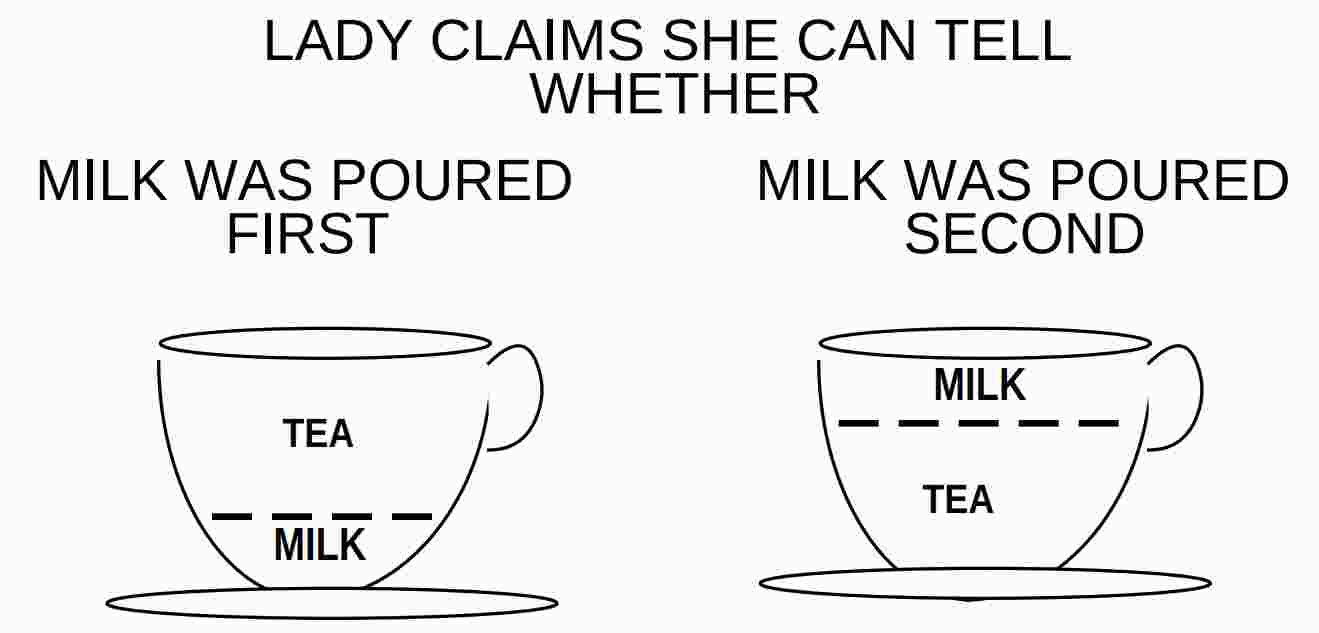
\includegraphics{images/teacups.jpg}
\caption{}
\end{figure}

\begin{Shaded}
\begin{Highlighting}[]
\KeywordTok{library}\NormalTok{(mosaic)}
\KeywordTok{rflip}\NormalTok{()}
\CommentTok{#> }
\CommentTok{#> Flipping 1 coin [ Prob(Heads) = 0.5 ] ...}
\CommentTok{#> }
\CommentTok{#> H}
\CommentTok{#> }
\CommentTok{#> Number of Heads: 1 [Proportion Heads: 1]}
\end{Highlighting}
\end{Shaded}

\begin{Shaded}
\begin{Highlighting}[]
\KeywordTok{rflip}\NormalTok{(}\DecValTok{10}\NormalTok{)}
\CommentTok{#> }
\CommentTok{#> Flipping 10 coins [ Prob(Heads) = 0.5 ] ...}
\CommentTok{#> }
\CommentTok{#> H T T T T H T T T H}
\CommentTok{#> }
\CommentTok{#> Number of Heads: 3 [Proportion Heads: 0.3]}
\end{Highlighting}
\end{Shaded}

\begin{Shaded}
\begin{Highlighting}[]
\NormalTok{mu =}\StringTok{ }\DecValTok{500}
\NormalTok{sigma =}\StringTok{ }\DecValTok{100}
\NormalTok{x =}\StringTok{ }\KeywordTok{rnorm}\NormalTok{(}\DecValTok{500}\NormalTok{, }\DataTypeTok{mean=}\NormalTok{mu, }\DataTypeTok{sd=}\NormalTok{sigma)}
\KeywordTok{favstats}\NormalTok{(x)}
\CommentTok{#>  min    Q1 median    Q3   max  mean    sd   n missing}
\CommentTok{#>  117 431.4  497.4 563.1 811.6 500.2 99.16 500       0}
\NormalTok{meanconfint =}\StringTok{ }\ControlFlowTok{function}\NormalTok{ (x, sigma, }\DataTypeTok{level =} \FloatTok{0.95}\NormalTok{, ...) \{}
\NormalTok{  se =}\StringTok{ }\NormalTok{sigma }\OperatorTok{/}\StringTok{ }\KeywordTok{sqrt}\NormalTok{(}\KeywordTok{length}\NormalTok{(x))}
\NormalTok{  mu =}\StringTok{ }\KeywordTok{mean}\NormalTok{(x)}
\NormalTok{  z =}\StringTok{ }\KeywordTok{qnorm}\NormalTok{(}\DecValTok{1} \OperatorTok{-}\StringTok{ }\NormalTok{(}\DecValTok{1} \OperatorTok{-}\StringTok{ }\NormalTok{level)}\OperatorTok{/}\DecValTok{2}\NormalTok{)}
\NormalTok{  out =}\StringTok{ }\KeywordTok{c}\NormalTok{(mu, mu }\OperatorTok{-}\StringTok{ }\NormalTok{z }\OperatorTok{*}\StringTok{ }\NormalTok{se, mu }\OperatorTok{+}\StringTok{ }\NormalTok{z }\OperatorTok{*}\StringTok{ }\NormalTok{se)}
  \KeywordTok{names}\NormalTok{(out) =}\StringTok{ }\KeywordTok{c}\NormalTok{(}\StringTok{"mean"}\NormalTok{, }\StringTok{"lower"}\NormalTok{, }\StringTok{"upper"}\NormalTok{)}
  \KeywordTok{return}\NormalTok{(out)}
\NormalTok{\}}
\KeywordTok{meanconfint}\NormalTok{(x, }\DataTypeTok{sigma =}\NormalTok{ sigma)}
\CommentTok{#>  mean lower upper }
\CommentTok{#> 500.2 491.4 509.0}
\NormalTok{randomx =}\StringTok{ }\KeywordTok{do}\NormalTok{(}\DecValTok{50}\NormalTok{) }\OperatorTok{*}\StringTok{ }\KeywordTok{rnorm}\NormalTok{(}\DecValTok{500}\NormalTok{, }\DataTypeTok{mean=}\NormalTok{mu, }\DataTypeTok{sd=}\NormalTok{sigma)}
\NormalTok{ci =}\StringTok{ }\KeywordTok{data.frame}\NormalTok{(}\KeywordTok{t}\NormalTok{(}\KeywordTok{apply}\NormalTok{(randomx, }\DecValTok{1}\NormalTok{, meanconfint, }\DataTypeTok{sigma=}\NormalTok{sigma, }\DataTypeTok{level=}\FloatTok{0.90}\NormalTok{)))}
\KeywordTok{head}\NormalTok{(ci, }\DecValTok{3}\NormalTok{)}
\CommentTok{#>    mean lower upper}
\CommentTok{#> 1 493.1 485.7 500.5}
\CommentTok{#> 2 492.8 485.5 500.2}
\CommentTok{#> 3 502.4 495.1 509.8}

\KeywordTok{xyplot}\NormalTok{(}\DecValTok{1}\OperatorTok{:}\KeywordTok{nrow}\NormalTok{(ci) }\OperatorTok{~}\StringTok{ }\NormalTok{mean, }\DataTypeTok{data=}\NormalTok{ci, }\DataTypeTok{xlim=}\KeywordTok{range}\NormalTok{(ci), }\DataTypeTok{xlab=}\StringTok{"SAT score"}\NormalTok{, }\DataTypeTok{ylab=}\StringTok{"Index"}\NormalTok{)}
\KeywordTok{ladd}\NormalTok{(}\KeywordTok{panel.abline}\NormalTok{(}\DataTypeTok{v=}\DecValTok{500}\NormalTok{, }\DataTypeTok{col=}\StringTok{"lightgray"}\NormalTok{, }\DataTypeTok{lty=}\DecValTok{2}\NormalTok{))}
\KeywordTok{ladd}\NormalTok{(}\KeywordTok{with}\NormalTok{(ci, }\KeywordTok{panel.arrows}\NormalTok{(}\DataTypeTok{x0 =}\NormalTok{ lower, }\DataTypeTok{y0=}\DecValTok{1}\OperatorTok{:}\KeywordTok{nrow}\NormalTok{(ci), }\DataTypeTok{y1=}\DecValTok{1}\OperatorTok{:}\KeywordTok{nrow}\NormalTok{(ci), }\DataTypeTok{cex=}\FloatTok{0.5}\NormalTok{,}
                           \DataTypeTok{x1=}\NormalTok{upper, }\DataTypeTok{code=}\DecValTok{3}\NormalTok{)))}

\KeywordTok{head}\NormalTok{(}\KeywordTok{t}\NormalTok{(}\KeywordTok{apply}\NormalTok{(randomx, }\DecValTok{1}\NormalTok{, meanconfint, }\DataTypeTok{sigma=}\NormalTok{sigma, }\DataTypeTok{level=}\FloatTok{0.9}\NormalTok{)), }\DecValTok{3}\NormalTok{)}
\CommentTok{#>       mean lower upper}
\CommentTok{#> [1,] 493.1 485.7 500.5}
\CommentTok{#> [2,] 492.8 485.5 500.2}
\CommentTok{#> [3,] 502.4 495.1 509.8}
\end{Highlighting}
\end{Shaded}

\begin{center}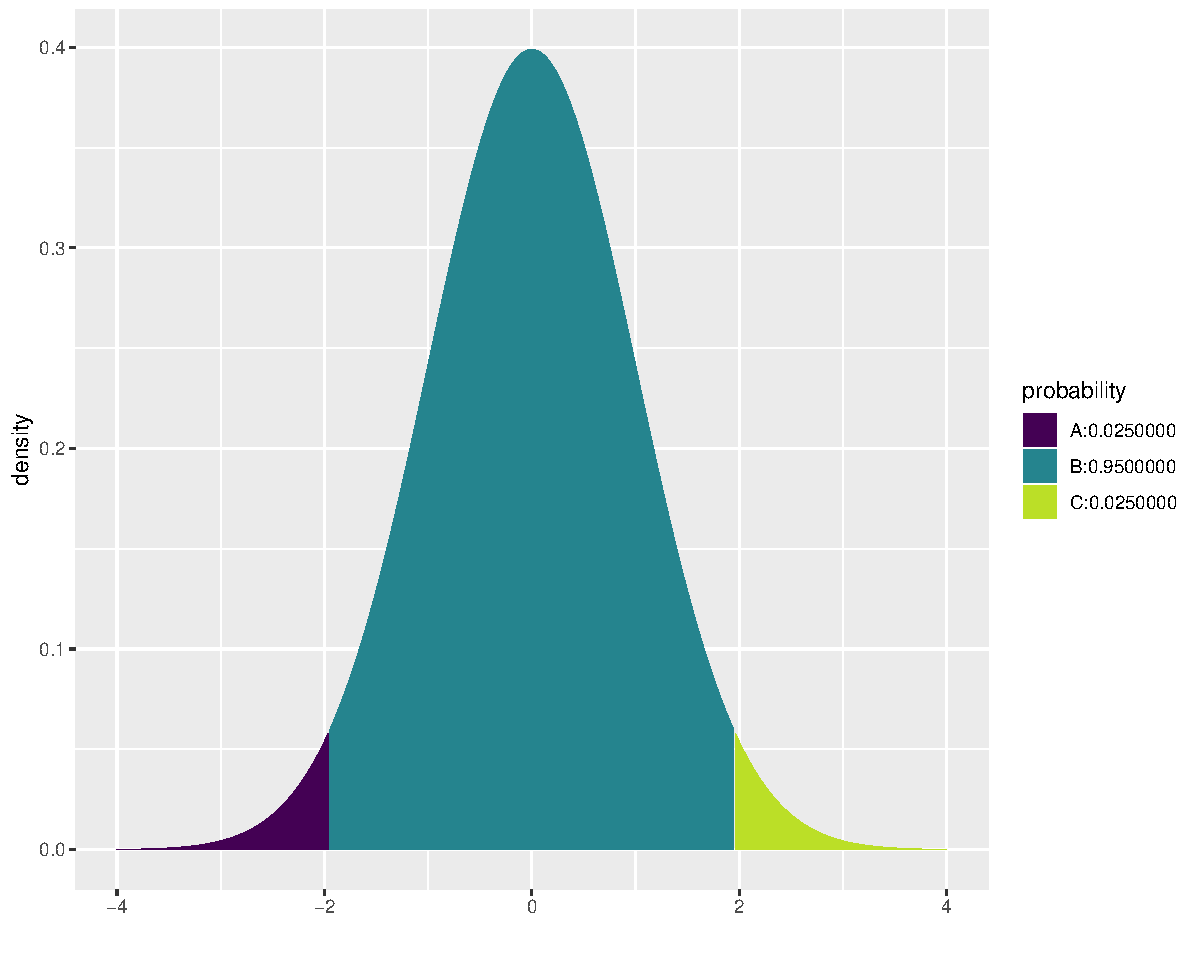
\includegraphics[width=\textwidth]{epib607_files/figure-latex/unnamed-chunk-18-1} 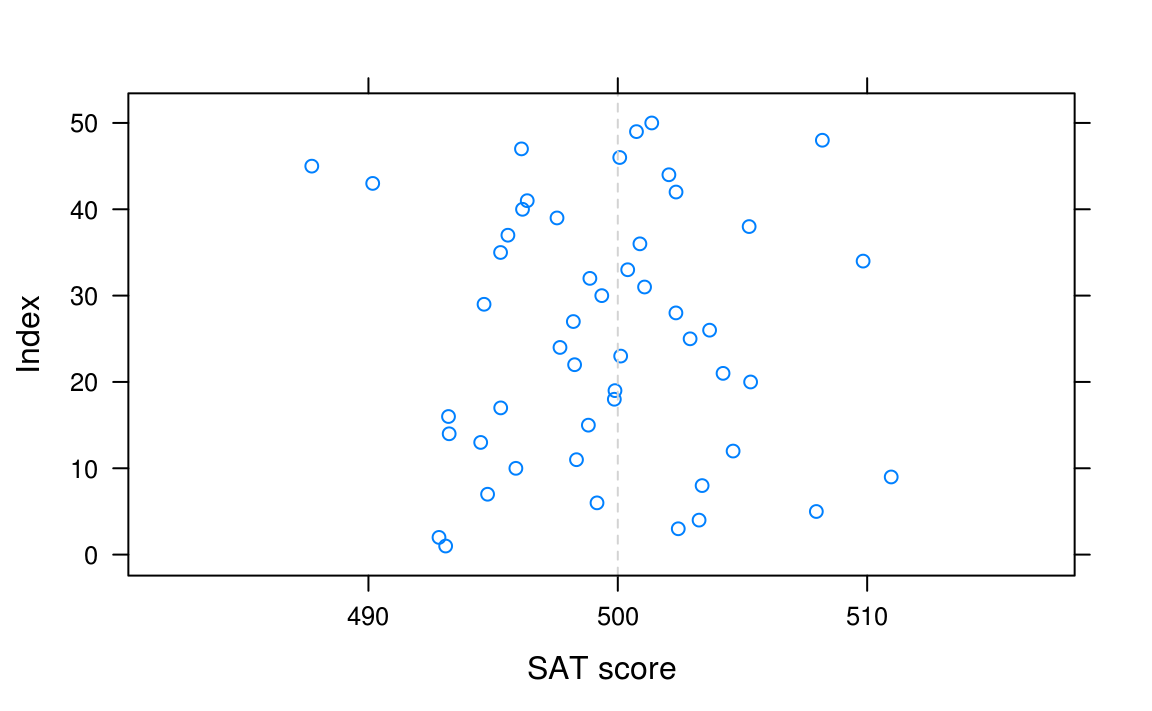
\includegraphics[width=\textwidth]{epib607_files/figure-latex/unnamed-chunk-18-2} 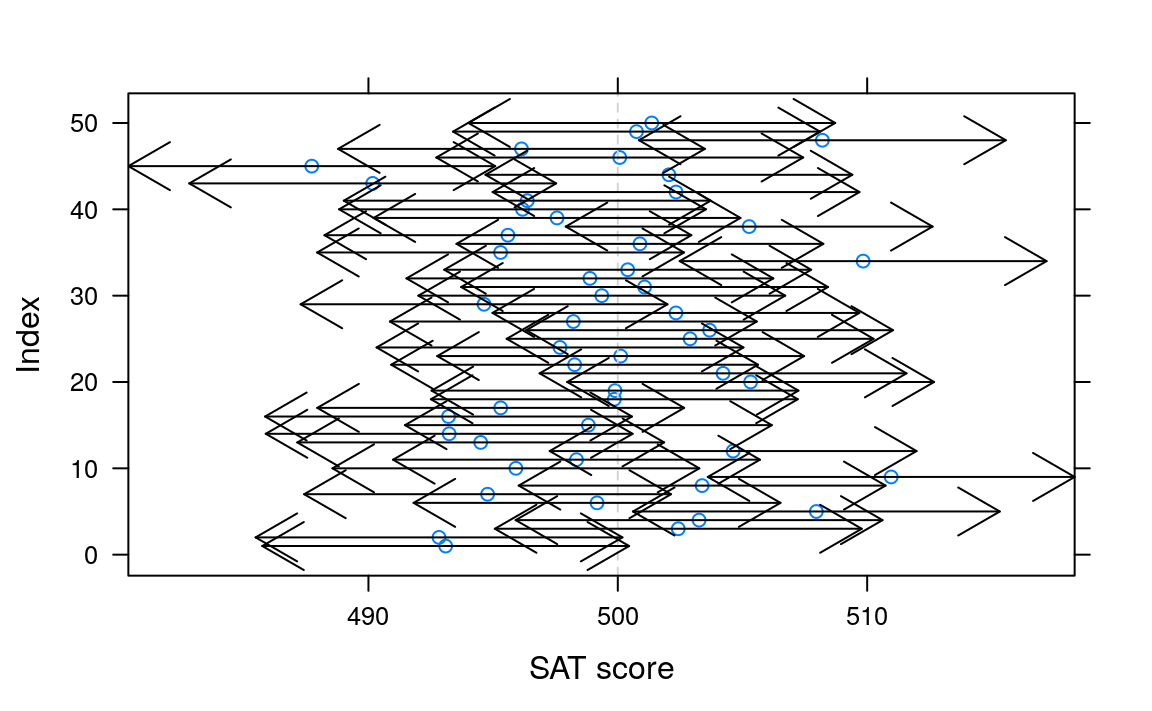
\includegraphics[width=\textwidth]{epib607_files/figure-latex/unnamed-chunk-18-3} \end{center}

\begin{Shaded}
\begin{Highlighting}[]
\NormalTok{T <-}\StringTok{ }\KeywordTok{chisq}\NormalTok{(substance }\OperatorTok{~}\StringTok{ }\KeywordTok{shuffle}\NormalTok{(sex), }\DataTypeTok{data =}\NormalTok{ HELPrct); T}
\CommentTok{#> X.squared }
\CommentTok{#>   0.07796}
\NormalTok{Substance.Null <-}\StringTok{ }\KeywordTok{do}\NormalTok{(}\DecValTok{999}\NormalTok{) }\OperatorTok{*}\StringTok{ }\KeywordTok{chisq}\NormalTok{(substance }\OperatorTok{~}\StringTok{ }\KeywordTok{shuffle}\NormalTok{(sex), }\DataTypeTok{data =}\NormalTok{ HELPrct)}
\KeywordTok{histogram}\NormalTok{( }\OperatorTok{~}\StringTok{ }\NormalTok{X.squared, }\DataTypeTok{data =}\NormalTok{ Substance.Null, }\DataTypeTok{v =}\NormalTok{ T, }\DataTypeTok{width =} \FloatTok{0.25}\NormalTok{)}
\KeywordTok{prop1}\NormalTok{( }\OperatorTok{~}\NormalTok{(X.squared }\OperatorTok{>=}\StringTok{ }\NormalTok{T), }\DataTypeTok{data =}\NormalTok{ Substance.Null)}
\CommentTok{#> prop_TRUE }
\CommentTok{#>     0.956}
\end{Highlighting}
\end{Shaded}

\begin{center}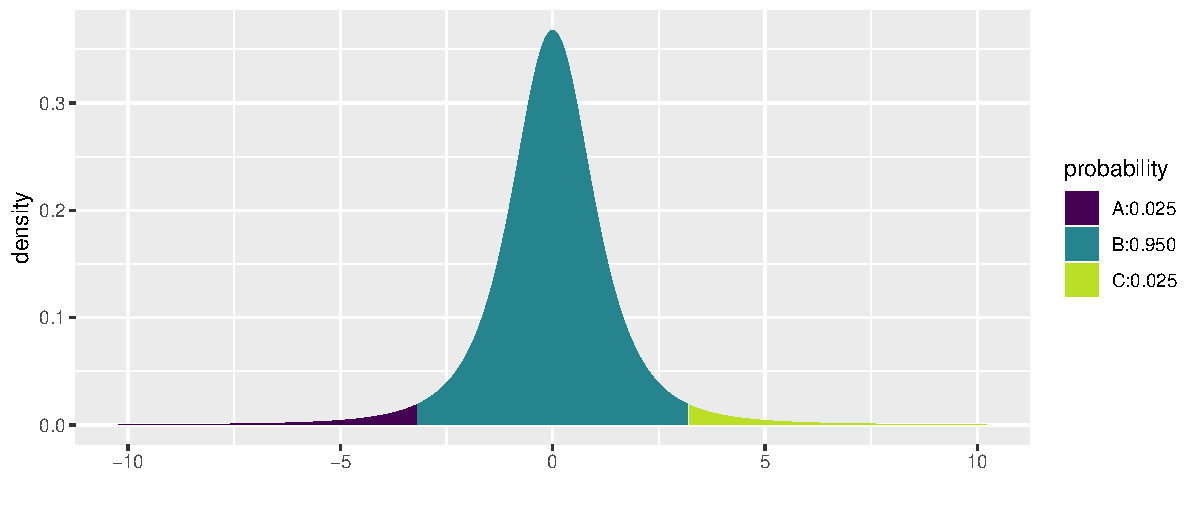
\includegraphics[width=\textwidth]{epib607_files/figure-latex/unnamed-chunk-19-1} \end{center}

\appendix


\chapter{Vectorization, *apply and for
loops}\label{vectorization-apply-and-for-loops}

This section will cover the basics of vectorizations, the
\texttt{*apply} family of functions and \texttt{for} loops.

\section{Vectorization}\label{vectorization}

Almost everything in \texttt{R} is a vector. A scalar is really a vector
of length 1 and a \texttt{data.frame} is a collection of vectors. An
nice feature of \texttt{R} is its vectorized capabilities. Vectorization
indicates that a function operates on a whole vector of values at the
same time and not just on a single value\footnote{\url{http://www.dummies.com/how-to/content/how-to-vectorize-your-functions-in-r.html}}.
If you have have ever taken a basic linear algebra course, this concept
will be familiar to you. \newline  \vspace{0.1in} Take for example two
vectors: \newline
\vspace{0.1in} \[
\begin{bmatrix} 1 \\ 2 \\ 3 \end{bmatrix} + 
\begin{bmatrix} 1 \\ 2 \\ 3 \end{bmatrix} =
\begin{bmatrix} 2 \\ 4 \\ 6 \end{bmatrix}
\] \newline  \vspace{0.1in} The corresponding \texttt{R} code is given
by:

\begin{Shaded}
\begin{Highlighting}[]
\NormalTok{a <-}\StringTok{ }\KeywordTok{c}\NormalTok{(}\DecValTok{1}\NormalTok{,}\DecValTok{2}\NormalTok{,}\DecValTok{3}\NormalTok{)}
\NormalTok{b <-}\StringTok{ }\KeywordTok{c}\NormalTok{(}\DecValTok{1}\NormalTok{,}\DecValTok{2}\NormalTok{,}\DecValTok{3}\NormalTok{)}
\NormalTok{a}\OperatorTok{+}\NormalTok{b}
\CommentTok{#> [1] 2 4 6}
\end{Highlighting}
\end{Shaded}

Many of the \texttt{base} functions in \texttt{R} are already
vectorized. Here are some common examples:

\begin{Shaded}
\begin{Highlighting}[]

\CommentTok{# generate a sequence of numbers from 1 to 10}
\NormalTok{(a <-}\StringTok{ }\DecValTok{1}\OperatorTok{:}\DecValTok{10}\NormalTok{)}
\CommentTok{#>  [1]  1  2  3  4  5  6  7  8  9 10}

\CommentTok{# sum the numbers from 1 to 10}
\KeywordTok{sum}\NormalTok{(a)}
\CommentTok{#> [1] 55}

\CommentTok{# calculate sums of each column}
\KeywordTok{colSums}\NormalTok{(iris[, }\OperatorTok{-}\DecValTok{5}\NormalTok{])}
\CommentTok{#> Sepal.Length  Sepal.Width Petal.Length  Petal.Width }
\CommentTok{#>        876.5        458.6        563.7        179.9}
\end{Highlighting}
\end{Shaded}

\begin{quote}
\textbf{Exercise}: What happens when you sum two vectors of different
lengths?
\end{quote}

\section{\texorpdfstring{Family of \texttt{*apply}
functions}{Family of *apply functions}}\label{family-of-apply-functions}

\begin{itemize}
\tightlist
\item
  \texttt{apply}, \texttt{lapply} and \texttt{sapply} are some of the
  most commonly used class of functions in \texttt{R}
\item
  \texttt{*apply} functions are not necessarily faster than loops, but
  can be easier to read (and vice cersa)
\item
  \texttt{apply} is used when you need to perform an operation on every
  row or column of a matrix or data.frame
\item
  \texttt{lapply} and \texttt{sapply} differ in the format of the
  output. The former returns a list while the ladder returns a vector
\item
  There are other \texttt{*apply} functions such as \texttt{tapply},
  \texttt{vapply} and \texttt{mapply} with similar functionality and
  purpose
\end{itemize}

\subsection{Loops vs.~Apply}\label{loops-vs.apply}

\begin{Shaded}
\begin{Highlighting}[]

\CommentTok{# Getting the row means of two columns}
\CommentTok{# Generate data}
\NormalTok{N <-}\StringTok{ }\DecValTok{10000}
\NormalTok{x1 <-}\StringTok{ }\KeywordTok{runif}\NormalTok{(N)}
\NormalTok{x2 <-}\StringTok{ }\KeywordTok{runif}\NormalTok{(N)}
\NormalTok{d <-}\StringTok{ }\KeywordTok{as.data.frame}\NormalTok{(}\KeywordTok{cbind}\NormalTok{(x1, x2))}
\KeywordTok{head}\NormalTok{(d)}
\CommentTok{#>        x1     x2}
\CommentTok{#> 1 0.57632 0.9615}
\CommentTok{#> 2 0.56474 0.1950}
\CommentTok{#> 3 0.07399 0.3001}
\CommentTok{#> 4 0.45387 0.3823}
\CommentTok{#> 5 0.37328 0.1197}
\CommentTok{#> 6 0.33132 0.9891}

\CommentTok{# Loop:}
\CommentTok{# create a vector to store the results in }
\NormalTok{rowMeanFor <-}\StringTok{ }\KeywordTok{vector}\NormalTok{(}\StringTok{"double"}\NormalTok{, N)}

\ControlFlowTok{for}\NormalTok{ (i }\ControlFlowTok{in} \KeywordTok{seq_len}\NormalTok{(N)) \{}
\NormalTok{        rowMeanFor[[i]] <-}\StringTok{ }\KeywordTok{mean}\NormalTok{(}\KeywordTok{c}\NormalTok{(d[i, }\DecValTok{1}\NormalTok{], d[i, }\DecValTok{2}\NormalTok{]))}
\NormalTok{\}}

\CommentTok{# Apply:}
\NormalTok{rowMeanApply <-}\StringTok{ }\KeywordTok{apply}\NormalTok{(d, }\DecValTok{1}\NormalTok{, mean)}

\CommentTok{# are the results equal}
\KeywordTok{all.equal}\NormalTok{(rowMeanFor,rowMeanApply)}
\CommentTok{#> [1] TRUE}
\end{Highlighting}
\end{Shaded}

\subsection{\texorpdfstring{Descriptive Statistics using
\texttt{*apply}}{Descriptive Statistics using *apply}}\label{descriptive-statistics-using-apply}

\begin{Shaded}
\begin{Highlighting}[]
\KeywordTok{data}\NormalTok{(women)}
\CommentTok{# data structure}
\KeywordTok{str}\NormalTok{(women)}
\CommentTok{#> 'data.frame':    15 obs. of  2 variables:}
\CommentTok{#>  $ height: num  58 59 60 61 62 63 64 65 66 67 ...}
\CommentTok{#>  $ weight: num  115 117 120 123 126 129 132 135 139 142 ...}

\CommentTok{# calculate the mean for each column}
\KeywordTok{apply}\NormalTok{(women, }\DecValTok{2}\NormalTok{, mean)}
\CommentTok{#> height weight }
\CommentTok{#>   65.0  136.7}

\CommentTok{# apply 'fivenum' function to each column}
\KeywordTok{vapply}\NormalTok{(women, fivenum, }\KeywordTok{c}\NormalTok{(}\StringTok{"Min."}\NormalTok{ =}\StringTok{ }\DecValTok{0}\NormalTok{, }\StringTok{"1st Qu."}\NormalTok{ =}\StringTok{ }\DecValTok{0}\NormalTok{, }\StringTok{"Median"}\NormalTok{ =}\StringTok{ }\DecValTok{0}\NormalTok{, }
                         \StringTok{"3rd Qu."}\NormalTok{ =}\StringTok{ }\DecValTok{0}\NormalTok{, }\StringTok{"Max."}\NormalTok{ =}\StringTok{ }\DecValTok{0}\NormalTok{))}
\CommentTok{#>         height weight}
\CommentTok{#> Min.      58.0  115.0}
\CommentTok{#> 1st Qu.   61.5  124.5}
\CommentTok{#> Median    65.0  135.0}
\CommentTok{#> 3rd Qu.   68.5  148.0}
\CommentTok{#> Max.      72.0  164.0}
\end{Highlighting}
\end{Shaded}

\subsection{\texorpdfstring{Creating new columns using
\texttt{sapply}}{Creating new columns using sapply}}\label{creating-new-columns-using-sapply}

You can apply a \emph{user defined function} to columns or the entire
data frame:

\begin{Shaded}
\begin{Highlighting}[]
\CommentTok{# the ouput of sapply is a vector}
\CommentTok{# the 's' in sapply stands for 'simplified' apply}
\NormalTok{mtcars}\OperatorTok{$}\NormalTok{gear2 <-}\StringTok{ }\KeywordTok{sapply}\NormalTok{(mtcars}\OperatorTok{$}\NormalTok{gear, }
                       \ControlFlowTok{function}\NormalTok{(i) }\ControlFlowTok{if}\NormalTok{ (i}\OperatorTok{==}\DecValTok{4}\NormalTok{) }\StringTok{"alot"} \ControlFlowTok{else} \StringTok{"some"}\NormalTok{)}

\KeywordTok{head}\NormalTok{(mtcars)[,}\KeywordTok{c}\NormalTok{(}\StringTok{"gear"}\NormalTok{,}\StringTok{"gear2"}\NormalTok{)]}
\CommentTok{#>                   gear gear2}
\CommentTok{#> Mazda RX4            4  alot}
\CommentTok{#> Mazda RX4 Wag        4  alot}
\CommentTok{#> Datsun 710           4  alot}
\CommentTok{#> Hornet 4 Drive       3  some}
\CommentTok{#> Hornet Sportabout    3  some}
\CommentTok{#> Valiant              3  some}
\end{Highlighting}
\end{Shaded}

\subsection{\texorpdfstring{Applying functions to subsets using
\texttt{tapply}}{Applying functions to subsets using tapply}}\label{applying-functions-to-subsets-using-tapply}

\begin{Shaded}
\begin{Highlighting}[]

\CommentTok{# Fisher's famous dataset }
\KeywordTok{data}\NormalTok{(iris)}
\KeywordTok{str}\NormalTok{(iris)}
\CommentTok{#> 'data.frame':    150 obs. of  5 variables:}
\CommentTok{#>  $ Sepal.Length: num  5.1 4.9 4.7 4.6 5 5.4 4.6 5 4.4 4.9 ...}
\CommentTok{#>  $ Sepal.Width : num  3.5 3 3.2 3.1 3.6 3.9 3.4 3.4 2.9 3.1 ...}
\CommentTok{#>  $ Petal.Length: num  1.4 1.4 1.3 1.5 1.4 1.7 1.4 1.5 1.4 1.5 ...}
\CommentTok{#>  $ Petal.Width : num  0.2 0.2 0.2 0.2 0.2 0.4 0.3 0.2 0.2 0.1 ...}
\CommentTok{#>  $ Species     : Factor w/ 3 levels "setosa","versicolor",..: 1 1 1 1 1 1 1 1 1 1 ...}

\CommentTok{# mean sepal length by species }
\KeywordTok{tapply}\NormalTok{(iris}\OperatorTok{$}\NormalTok{Sepal.Length, iris}\OperatorTok{$}\NormalTok{Species, mean)}
\CommentTok{#>     setosa versicolor  virginica }
\CommentTok{#>      5.006      5.936      6.588}
\end{Highlighting}
\end{Shaded}

\subsection{\texorpdfstring{Nested for loops using
\texttt{mapply}}{Nested for loops using mapply}}\label{nested-for-loops-using-mapply}

\texttt{mapply} is my favorite \texttt{base} \texttt{R} function and
here are some reasons why:

\begin{itemize}
\tightlist
\item
  Using \texttt{mapply} is equivalent to writing nested \texttt{for}
  loops except that it is 100\% more human readable and less prone to
  errors
\item
  It is an effective way of conducting simulations because it iterates
  of many arguments
\end{itemize}

Let's say you want to generate random samples from a normal distribution
with varying means and standard deviations. Of course the brute force
way would be to write out the command once, copy paste as many times as
you want, and then manually change the arguments for \texttt{mean} and
\texttt{sd} in the \texttt{rnorm} function as so:

\begin{Shaded}
\begin{Highlighting}[]
\NormalTok{v1 <-}\StringTok{ }\KeywordTok{rnorm}\NormalTok{(}\DecValTok{100}\NormalTok{, }\DataTypeTok{mean =} \DecValTok{5}\NormalTok{, }\DataTypeTok{sd =} \DecValTok{1}\NormalTok{)}
\NormalTok{v2 <-}\StringTok{ }\KeywordTok{rnorm}\NormalTok{(}\DecValTok{100}\NormalTok{, }\DataTypeTok{mean =} \DecValTok{10}\NormalTok{, }\DataTypeTok{sd =} \DecValTok{5}\NormalTok{)}
\NormalTok{v3 <-}\StringTok{ }\KeywordTok{rnorm}\NormalTok{(}\DecValTok{100}\NormalTok{, }\DataTypeTok{mean =} \OperatorTok{-}\DecValTok{3}\NormalTok{, }\DataTypeTok{sd =} \DecValTok{10}\NormalTok{)}
\end{Highlighting}
\end{Shaded}

This isn't too bad for three vectors. But what if you want to generate
many more combinations of means and sds ? Furthermore, how can you keep
track of the parameters you used? Now lets consider the \texttt{mapply}
function:

\begin{Shaded}
\begin{Highlighting}[]
\NormalTok{means <-}\StringTok{ }\KeywordTok{c}\NormalTok{(}\DecValTok{5}\NormalTok{,}\DecValTok{10}\NormalTok{,}\OperatorTok{-}\DecValTok{3}\NormalTok{) ; sds <-}\StringTok{ }\KeywordTok{c}\NormalTok{(}\DecValTok{1}\NormalTok{,}\DecValTok{5}\NormalTok{,}\DecValTok{10}\NormalTok{) }

\CommentTok{# MoreArgs is a list of arguments that dont change}
\NormalTok{randomNormals <-}\StringTok{ }\KeywordTok{mapply}\NormalTok{(rnorm, }\DataTypeTok{mean =}\NormalTok{ means, }\DataTypeTok{sd =}\NormalTok{ sds, }
                        \DataTypeTok{MoreArgs =} \KeywordTok{list}\NormalTok{(}\DataTypeTok{n =} \DecValTok{100}\NormalTok{))}

\KeywordTok{head}\NormalTok{(randomNormals)}
\CommentTok{#>       [,1]   [,2]    [,3]}
\CommentTok{#> [1,] 3.836  8.771   5.144}
\CommentTok{#> [2,] 4.525  9.376  -2.280}
\CommentTok{#> [3,] 4.072 13.144   2.940}
\CommentTok{#> [4,] 4.737 18.210 -13.118}
\CommentTok{#> [5,] 5.690 22.951  -7.008}
\CommentTok{#> [6,] 4.826  7.615 -15.323}
\end{Highlighting}
\end{Shaded}

The following diagram (from
\href{http://r4ds.had.co.nz/iteration.html\#mapping-over-multiple-arguments}{r4ds})
describes exactly what is going on in the above function call to
\texttt{mapply}:

\begin{figure}
\centering
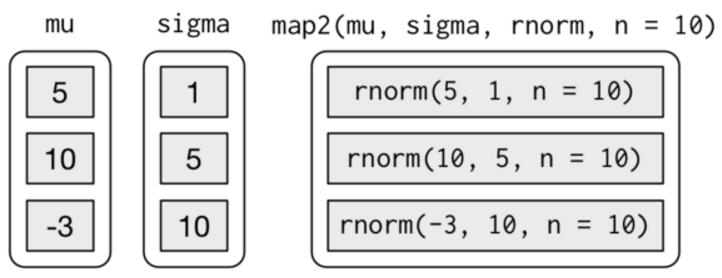
\includegraphics{images/mapply.png}
\caption{}
\end{figure}

Advantages:

\begin{enumerate}
\def\labelenumi{\arabic{enumi}.}
\tightlist
\item
  Result is automatically stored in a matrix
\item
  The parameters are also saved in \texttt{R} objects so that they can
  be easily manipulated and/or recovered
\end{enumerate}

Consider a more complex scenario where you want to consider many
possible combinations of means and sds. We take advantage of the
\texttt{expand.grid} function to create a \texttt{data.frame} of
simulation parameters:

\begin{Shaded}
\begin{Highlighting}[]
\NormalTok{simParams <-}\StringTok{ }\KeywordTok{expand.grid}\NormalTok{(}\DataTypeTok{means =} \DecValTok{1}\OperatorTok{:}\DecValTok{10}\NormalTok{,}
                         \DataTypeTok{sds =} \DecValTok{1}\OperatorTok{:}\DecValTok{10}\NormalTok{)}

\NormalTok{randomNormals <-}\StringTok{ }\KeywordTok{mapply}\NormalTok{(rnorm, }\DataTypeTok{mean =}\NormalTok{ simParams}\OperatorTok{$}\NormalTok{means, }
                        \DataTypeTok{sd =}\NormalTok{ simParams}\OperatorTok{$}\NormalTok{sds, }
                        \DataTypeTok{MoreArgs =} \KeywordTok{list}\NormalTok{(}\DataTypeTok{n =} \DecValTok{100}\NormalTok{))}

\KeywordTok{dim}\NormalTok{(randomNormals)}
\CommentTok{#> [1] 100 100}
\end{Highlighting}
\end{Shaded}

\section{\texorpdfstring{Creating dynamic documents with
\texttt{mapply}}{Creating dynamic documents with mapply}}\label{creating-dynamic-documents-with-mapply}

\texttt{mapply} together with the \texttt{rmarkdown} package
\citep{R-rmarkdown} can be very useful to create dynamic documents for
exploratory analysis. We illustrate this using the Motor Trend Car Road
Tests data which comes pre-loaded in \texttt{R}.

\begin{quote}
The data was extracted from the 1974 Motor Trend US magazine, and
comprises fuel consumption and 10 aspects of automobile design and
performance for 32 automobiles (1973--74 models).
\end{quote}

Copy the code below in a file called \texttt{mapplyRmarkdown.Rmd} :

Copy the code below in a file called \texttt{boxplotTemplate} :

\chapter{Appendix B}\label{appendix-b}

\bibliography{bib/book.bib,bib/packages.bib}


\end{document}
